% Options for packages loaded elsewhere
\PassOptionsToPackage{unicode}{hyperref}
\PassOptionsToPackage{hyphens}{url}
\PassOptionsToPackage{dvipsnames,svgnames,x11names}{xcolor}
%
\documentclass[
  authoryear,
  preprint,
  3p,
  twocolumn]{elsarticle}

\usepackage{amsmath,amssymb}
\usepackage{iftex}
\ifPDFTeX
  \usepackage[T1]{fontenc}
  \usepackage[utf8]{inputenc}
  \usepackage{textcomp} % provide euro and other symbols
\else % if luatex or xetex
  \usepackage{unicode-math}
  \defaultfontfeatures{Scale=MatchLowercase}
  \defaultfontfeatures[\rmfamily]{Ligatures=TeX,Scale=1}
\fi
\usepackage{lmodern}
\ifPDFTeX\else  
    % xetex/luatex font selection
\fi
% Use upquote if available, for straight quotes in verbatim environments
\IfFileExists{upquote.sty}{\usepackage{upquote}}{}
\IfFileExists{microtype.sty}{% use microtype if available
  \usepackage[]{microtype}
  \UseMicrotypeSet[protrusion]{basicmath} % disable protrusion for tt fonts
}{}
\makeatletter
\@ifundefined{KOMAClassName}{% if non-KOMA class
  \IfFileExists{parskip.sty}{%
    \usepackage{parskip}
  }{% else
    \setlength{\parindent}{0pt}
    \setlength{\parskip}{6pt plus 2pt minus 1pt}}
}{% if KOMA class
  \KOMAoptions{parskip=half}}
\makeatother
\usepackage{xcolor}
\setlength{\emergencystretch}{3em} % prevent overfull lines
\setcounter{secnumdepth}{5}
% Make \paragraph and \subparagraph free-standing
\ifx\paragraph\undefined\else
  \let\oldparagraph\paragraph
  \renewcommand{\paragraph}[1]{\oldparagraph{#1}\mbox{}}
\fi
\ifx\subparagraph\undefined\else
  \let\oldsubparagraph\subparagraph
  \renewcommand{\subparagraph}[1]{\oldsubparagraph{#1}\mbox{}}
\fi


\providecommand{\tightlist}{%
  \setlength{\itemsep}{0pt}\setlength{\parskip}{0pt}}\usepackage{longtable,booktabs,array}
\usepackage{calc} % for calculating minipage widths
% Correct order of tables after \paragraph or \subparagraph
\usepackage{etoolbox}
\makeatletter
\patchcmd\longtable{\par}{\if@noskipsec\mbox{}\fi\par}{}{}
\makeatother
% Allow footnotes in longtable head/foot
\IfFileExists{footnotehyper.sty}{\usepackage{footnotehyper}}{\usepackage{footnote}}
\makesavenoteenv{longtable}
\usepackage{graphicx}
\makeatletter
\def\maxwidth{\ifdim\Gin@nat@width>\linewidth\linewidth\else\Gin@nat@width\fi}
\def\maxheight{\ifdim\Gin@nat@height>\textheight\textheight\else\Gin@nat@height\fi}
\makeatother
% Scale images if necessary, so that they will not overflow the page
% margins by default, and it is still possible to overwrite the defaults
% using explicit options in \includegraphics[width, height, ...]{}
\setkeys{Gin}{width=\maxwidth,height=\maxheight,keepaspectratio}
% Set default figure placement to htbp
\makeatletter
\def\fps@figure{htbp}
\makeatother

\makeatletter
\makeatother
\makeatletter
\makeatother
\makeatletter
\@ifpackageloaded{caption}{}{\usepackage{caption}}
\AtBeginDocument{%
\ifdefined\contentsname
  \renewcommand*\contentsname{Table of contents}
\else
  \newcommand\contentsname{Table of contents}
\fi
\ifdefined\listfigurename
  \renewcommand*\listfigurename{List of Figures}
\else
  \newcommand\listfigurename{List of Figures}
\fi
\ifdefined\listtablename
  \renewcommand*\listtablename{List of Tables}
\else
  \newcommand\listtablename{List of Tables}
\fi
\ifdefined\figurename
  \renewcommand*\figurename{Figura}
\else
  \newcommand\figurename{Figura}
\fi
\ifdefined\tablename
  \renewcommand*\tablename{Table}
\else
  \newcommand\tablename{Table}
\fi
}
\@ifpackageloaded{float}{}{\usepackage{float}}
\floatstyle{ruled}
\@ifundefined{c@chapter}{\newfloat{codelisting}{h}{lop}}{\newfloat{codelisting}{h}{lop}[chapter]}
\floatname{codelisting}{Listing}
\newcommand*\listoflistings{\listof{codelisting}{List of Listings}}
\makeatother
\makeatletter
\@ifpackageloaded{caption}{}{\usepackage{caption}}
\@ifpackageloaded{subcaption}{}{\usepackage{subcaption}}
\makeatother
\makeatletter
\@ifpackageloaded{tcolorbox}{}{\usepackage[skins,breakable]{tcolorbox}}
\makeatother
\makeatletter
\@ifundefined{shadecolor}{\definecolor{shadecolor}{rgb}{.97, .97, .97}}
\makeatother
\makeatletter
\makeatother
\makeatletter
\makeatother
\usepackage{float}
\makeatletter
\let\oldlt\longtable
\let\endoldlt\endlongtable
\def\longtable{\@ifnextchar[\longtable@i \longtable@ii}
\def\longtable@i[#1]{\begin{figure}[H]
\onecolumn
\begin{minipage}{0.5\textwidth}
\oldlt[#1]
}
\def\longtable@ii{\begin{figure}[H]
\onecolumn
\begin{minipage}{0.5\textwidth}
\oldlt
}
\def\endlongtable{\endoldlt
\end{minipage}
\twocolumn
\end{figure}}
\makeatother
\journal{Journal of Sea Research}
\ifLuaTeX
  \usepackage{selnolig}  % disable illegal ligatures
\fi
\usepackage[]{natbib}
\bibliographystyle{elsarticle-harv}
\IfFileExists{bookmark.sty}{\usepackage{bookmark}}{\usepackage{hyperref}}
\IfFileExists{xurl.sty}{\usepackage{xurl}}{} % add URL line breaks if available
\urlstyle{same} % disable monospaced font for URLs
\hypersetup{
  pdftitle={Diferencias en la composición de sustrato entre Dzilam de Bravo y El Cuyo de la península de Yucatán},
  pdfauthor={Sebastián Medina; David Sánchez; Diego Muñoz},
  pdfkeywords={Sustrato, Megabentos, Pastos marinos, Zona submareal},
  colorlinks=true,
  linkcolor={blue},
  filecolor={Maroon},
  citecolor={Blue},
  urlcolor={Blue},
  pdfcreator={LaTeX via pandoc}}

\setlength{\parindent}{6pt}
\begin{document}

\begin{frontmatter}
\title{Diferencias en la composición de sustrato entre Dzilam de Bravo y
El Cuyo de la península de Yucatán}
\author[1]{Sebastián Medina%
\corref{cor1}%
}
 \ead{319529818@enesmerida.unam.mx} 
\author[1]{David Sánchez%
%
}
 \ead{420049609@enesmerida.unam.mx} 
\author[1]{Diego Muñoz%
%
}
 \ead{317137150@enesmerida.unam.mx} 

\affiliation[1]{organization={ENES UNAM unidad Mérida, Ecología de Campo
VI},addressline={Tablaje Catastral N°6998, Carretera Mérida-Tetiz Km.
4.5},city={Ucú},postcode={97357},postcodesep={}}

\cortext[cor1]{Corresponding author}



        
\begin{abstract}
Los pastos marinos tienen una amplia distribución alrededor de la
península de Yucatán y representan un pilar destacado para el
sostenimiento de la fauna bentónica. No obstante, dicha distribución no
es igual ni a lo largo de la costa ni mar adentro. A través de una
versión modificada de la metodología AGRRA, caracterizamos y comparamos
la composición de sustratos submareales entre dos localidades del norte
de la península de Yucatán (Dzilam de Bravo y El Cuyo) a 20, 40 y 60
metros de la línea de costa. También exploramos la probabilidad de
detección de la fauna macrobentónica en ambas localidades. Encontramos
que, al menos en los primeros 60 metros de zona submareal, Dzilam de
Bravo presenta una mayor diversidad de sustratos que El Cuyo y que estos
varían en su composición en función de la distancia a la línea de costa.
De los nueve sustratos registrados para Dzilam de Bravo, dos fueron
especies de pastos marinos: \emph{Thalassia testudinum} y
\emph{Syringodium filiforme}; creemos que la dominancia de la segunda
indica procesos de sucesión ecológica temprana en la localidad. Por otro
lado, la probabilidad de detección de fauna bentónica fue baja para
Dzilam de Bravo (0.11 para bivalvos y 0.22 para gasterópodos) y nula
para el Cuyo. Nuestros hallazgos secundan la heterogeneidad reportada en
sustratos de pastos marinos a lo largo de la península de Yucatán.
\end{abstract}





\begin{keyword}
    Sustrato \sep Megabentos \sep Pastos marinos \sep 
    Zona submareal
\end{keyword}
\end{frontmatter}
    \ifdefined\Shaded\renewenvironment{Shaded}{\begin{tcolorbox}[sharp corners, frame hidden, boxrule=0pt, borderline west={3pt}{0pt}{shadecolor}, enhanced, interior hidden, breakable]}{\end{tcolorbox}}\fi

\hypertarget{introducciuxf3n}{%
\section{Introducción}\label{introducciuxf3n}}

Las zonas costeras representan un foco de interés para la biodiversidad,
pues son la base de intercambio de materia biótica y abiótica entre los
ecosistemas terrestres y los marinos. Estas albergan una gran diversidad
de especies en los ecosistemas que la conforman, como los pastos
marinos. Estos están constituidos, principalmente, por una comunidad
vegetal bentónica \citep{herrera2019pastos} y se distribuyen~a manera de
parches estratificados.

Para el caso de la península de Yucatán, se ha reportado una amplia
distribución de especies de pastos marinos, como \emph{Thalassia
testudinum, Halodule wrightii}, \emph{Syringodium filiforme} y
\emph{Ruppia mexicana,} por mencionar algunas, siendo esta última una
especie éndemica de la región \citep{unknown}. Tal fenómeno se ha
explicado por la poca profundidad que tienen sus costas, lo cual permite
niveles de irradiación óptimos para los mismos en~ regiones vastas.
Además, Sánchez et al \citep{sanchez2007analisis} propone que la
composición calcárea del sustrato favorece la fijación y colonización de
las plantas macrófitas, lo que propicia el crecimiento de una variada
macroflora marina.

Los pastos marinos cumplen con diferentes servicios ecosistémicos como,
la captura de carbono, disipación de corrientes (lo que permite la
estructuración de las costas), reducción de las tasas de erosión costera
\citep{herrera2019pastos} y provisión de microhábitats para una gran
diversidad de organismos invertebrados considerados cómo fauna
bentónica. La fauna bentónica es toda aquella que se encuentra en el
fondo del agua y ha sido clasificada en diferentes tamaños:
microbentónica \textless0.063 mm, meiobentónica 0.063--1.0 mm,
macrobentónica \textgreater1.0 mm y megabentónica \textgreater{} 10.0 mm
\citep{tagliapietra2010benthic}. Organismos como oligoquetos,
poliquetos, moluscos, gasterópodos, bivalvos, crustáceos, etc., realizan
funciones importantes dentro de~ su ecosistema.~ Algunos cumplen con el
papel de ser organismos detritívoros, otros como filtradores de materia
orgánica y demás. Asimismo, también están ligados a redes tróficas como
alimento para especies de mayor tamaño \citep{tagliapietra2010benthic}.

Continuar estudiando la composición de las zonas bentónicas submareales
es una tarea importante a realizar, ya que, de esta manera poder evaluar
y comprender los procesos ecológicos que se desarrollan en esos
ecosistemas en vistas de mejorar planes de manejo para la biodiversidad
marina. Es en este contexto que el propósito de nuestro trabajo es
caracterizar la composición del sustrato submareal y la composición de
fauna megabentónica en dos localidades, Dzilam de Bravo y El Cuyo a 20 ,
40 y 60 metros de la línea de costa. con el objetivo de comparar ambos
sitios utilizando una metodología AGRRA.

\hypertarget{metodologuxeda}{%
\section{Metodología}\label{metodologuxeda}}

\hypertarget{uxe1rea-de-estudio}{%
\subsection{\texorpdfstring{\emph{Área de
estudio}}{Área de estudio}}\label{uxe1rea-de-estudio}}

En este estudio contemplamos a Dzilam de Bravo y El Cuyo. El primero,
situado en el norte de Yucatán entre los paralelos 21°19' y 21°32' N y
los meridianos 88°35' y 88°58', limita al norte con el Golfo de México y
está influenciado en su circulación oceánica por los vientos y las
corrientes provenientes del canal de Yucatán, principalmente
\citep{1834/36164}. Además, presenta una diversidad de fondos en la que
se encuentran fondos arenosos, arenosos con conchuela, duros de lajas y
piedras \citep{1834/36164}. Por su parte, El Cuyo se sitúa en el
paralelo 21°31' N y el meridiano 87°39', ubicado al noreste de la
península \citep{cnarioCuyo}. La costa presenta una pendiente reducida
con arenas combinadas de tamñaos medianos y pequeños, las corrientes
llevan una dirección Oeste-Noroeste, con velocidad promedio entre 0.7 y
0.8 nudos, alcanzando velocidades máximas de hasta 3 nudos
\citep{cnarioCuyo} (figura 1).

\hypertarget{descripciuxf3n-de-muxe9todos-de-campo}{%
\subsection{\texorpdfstring{\emph{Descripción de métodos de
campo}}{Descripción de métodos de campo}}\label{descripciuxf3n-de-muxe9todos-de-campo}}

\begin{figure}

{\centering \includegraphics{Mapa_dots3.jpg}

}

\caption{Mapa del área de estudio de Dzilam de bravo (figura superior
izquierda) y El Cuyo (figura superior derecha) y los sitios de
muestreo.}

\end{figure}

Empleando una versión modificada del protocolo AGRRA 2016-09-22 (Lang,
2016) para sustratos distintos a corales, demarcamos tres lineas de
muestreo paralelas a la playa, teniendo una separación de 20 m entre
cada una, dando una distancia total de 60 m a línea de costa. Cada línea
de muestreo contuvo tres transectos de 10 m separados por una distancia
de 20 m entre ellos; cada transecto fue marcado cada 10 cm a través de
una soga. Para la caracterización del sustrato, ocupamos una cámara Go
Pro versión 8 para grabar un video por transecto desde el inicio hasta
el final de la soga en el que se pudieran apreciar las marcas.
Posteriormente, tomamos en cuenta lo que yaciera cada 10 cm por debajo
de las marcas, identificamos el sustrato, según la composición las
especies vegetales asociadas al mismo. Por otro lado, para la
caracterización del megabentos submareal, ocupamos un cuadrante de 25 x
25 cm que colocamos en los metros 1, 3, 5, 7 y 9 de cada transecto y
aplicado a cada una de las distancias 20 m, 40 m y 60 m,
respectivamente. Dentro de cada uno de estos, observamos detenidamente
entre las macroalgas en búsqueda de animales bentónicos y registramos
tal acción en un video de 30 segundos como mínimo.

\hypertarget{procesamiento-de-datos}{%
\subsection{\texorpdfstring{\emph{Procesamiento de
datos}}{Procesamiento de datos}}\label{procesamiento-de-datos}}

Con los datos obtenidos mediante el protocolo de muestreo calculamos el
porcentaje de cobertura de diferentes especies de plantas marinas y
macroalgas para cada distancia de la costa. Posteriormente
estandarizamos los porcentajes (raíz cuarta) utilizando RStudio (versión
4.3.1). Despues se calculó una matriz de disimilitud de Bray-Curtis con
el paquete vegan \citep{manualR}, con la cual se realizó un análisis de
escalamiento multidimensional (MDS) no métrico con la paqueteria MASS
\citep{BookR}.

\hypertarget{resultados}{%
\section{Resultados}\label{resultados}}

\begin{figure}

{\centering 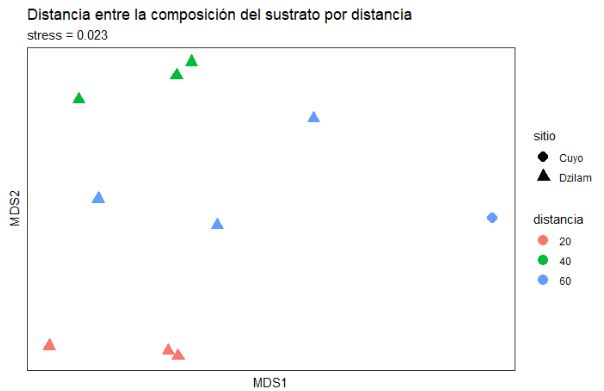
\includegraphics{MDS.JPG}

}

\caption{Composición del sustrato por distancia. Dzilam de Bravo
(triángulo); El Cuyo (círculo).}

\end{figure}

Las variables consideradas fueron tipos de sustrato por localidad y por
sitio, profundidad inicial por sitio y probabilidad de detección de
fauna bentónica por localidad.

Como se observa en la Figura 2, registramos una mayor diversidad de
sustratos en Dzilam de Bravo que en EL Cuyo. Estos varían parecen variar
en su composición en función de la distancia a la línea de costa. Se
aprecia que los sitios de las líneas de muestreo a 20 y 40 m son más
similares entre sí que aquellos del sitio 60 m. Respecto a la
profundidad del agua, ésta no fue muy disímil entre ambos sitios. Dzilam
de Bravo, contó con 0.5, 1.4 y 1.53 metros de profundidad para los
sitios 20, 40 y 60 metros, respectivamente. Por su parte, en El Cuyo se
registró 0.7 m, 1.2 m y 2 m de profundidad.

\begin{figure}

{\centering \includegraphics{Promedio_sus_gen.jpg}

}

\caption{Promedio general de sustratos de Dzilam de Bravo (azul) y El
Cuyo (rojo).}

\end{figure}

\begin{figure}

{\centering 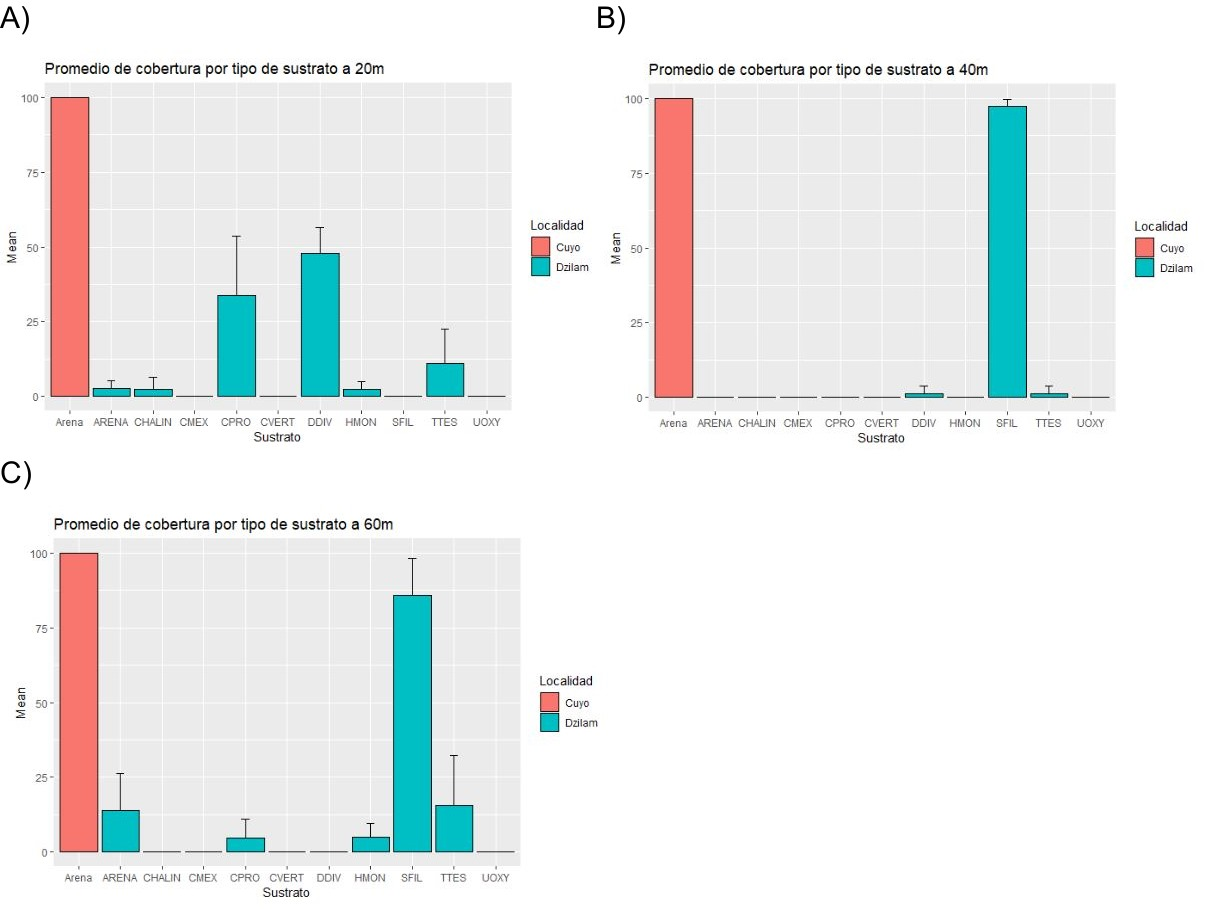
\includegraphics{Promedio_sustratos.JPG}

}

\caption{Cobertura de sustratos de Dzilam de Bravo (azul) y El Cuyo
(rojo). A) Distancia de 20 m de la línea de costa; B) Distancia de 40 m
de la línea de costa; C) Distancia de 60 m de la línea de costa.}

\end{figure}

En torno a la diversidad de sustratos por localidad ((figura 3), Dzilam
de Bravo, estuvo representada por dos especies de pastos marinos
(Thalassia testudinum y Syringodium filiforme) y siete especies de
macroalgas (\emph{Dictyota divaricata, Chaetomorpha linum, Halimeda
monile, Caulerpa verticillata, Caulerpa prolifera, Caulerpa mexicana} y
\emph{Ulvaria oxysperma}), mientras que El Cuyo solo presentó arena.
Cabe destacar pero hemos considerado \emph{D. divaricata} (aún cuando la
misma no está directamente asociada al sustrato) por su elevada
cobertura. Ahora bien, respecto a la dominancia de tales sustratos en el
sitio, se puede apreciar en la figura 4 que el sustrato con mayor
cobertura fue \emph{S. filiforme}, seguido por \emph{D.divaricata}. No
obstante, tal proporción difirió por sitio. El sitio a 20 metros fue
dominado por \emph{D. divaricata} seguida por \emph{C. prolifera}, el
sitio a 40 metros por \emph{S. filiforme} casi por completo y el sitio a
60 metros por \emph{S. filiforme} seguida por \emph{T. testudinum}.

\begin{figure}

{\centering \includegraphics{Especies_algas.JPG}

}

\caption{Vegetación bentónica de Dzilam de Bravo. A) \emph{Halimeda
monile}; B) \emph{Thalassia testudinum}; C) \emph{Syringodium
filifiorme}; D) \emph{Chaetomorpha linum}; E) \emph{Caulerpa
prolifera.}}

\end{figure}

Finalmente, respecto al megabentos en Dzilam de Bravo, la probabilidad
de detección de bivalvos fue de 0.11 mientras aquella de gasterópodos
fue de 0.22. Cabe destacar que sólo obtuvimos valores para estos grupos
dado que no registramos otros taxones. Por su parte, no hubo registro de
ningún organismo en El Cuyo.

\hypertarget{discusiuxf3n}{%
\section{Discusión}\label{discusiuxf3n}}

Las diferencias en la composición del sustrato entre Dzilam de Bravo y
El Cuyo son amplias, pues los resultados parecen reflejar tanto una
mayor diversidad en las especies asociadas al sustrato como una mayor
variación entre estas en función de la distancia a la línea de costa. En
este marco, mientras que en Dzilam de Bravo se registraron dos especies
de plantas marinas y siete especies de algas, en El Cuyo el único
sustrato registrado fue arena. Inicialmente, parecería que nuestros
resultados son contradictorios con la diversidad de macroalgas
reportadas en El Cuyo por Aguilar-Trujillo, et al.
\citep{aguilar2014variacion} o los pastos marinos identificados en el
norte de la Península por Herrera-Silveira et al.~en el libro de
Biodiversidad y Desarrollo humano de Yucatán
\citep{garcia2010biodiversidad}. No obstante, es posible que las
distancias que hemos considerado en el muestreo de El Cuyo no hayan sido
suficientes para abarcar zonas submareales con sustratos distintos a la
arena. Por tanto, a partir de nuestros resultados, no podemos concluir
información más allá de que en los primeros 60 m a partir de la línea de
costa, el Cuyo cuenta con arena como sustrato único mientras que en
Dzilam de Bravo existe una diversidad de sustratos constituida por
pastos marinos y macroalgas.

Las causas para tal contraste entre ambos sitios pueden ser variadas.
Debiéndose al establecimiento de la vegetación acuática, Calva-Benítez y
Torres Alvarado \citep{calva2011carbono} refieren que tanto la cobertura
como la distribución de ésta yacen determinadas por la salinidad, la
luz, la temperatura, el tipo de sedimento, la fuerza del viento y la
cantidad de materia orgánica disuelta y particulada. Por su parte,
Robbins y Bell \citep{robbins2000dynamics} sugieren que la distribución
de los pastos marinos también puede ser explicada por: características
fisiológicas y de crecimiento, impactos del pastoreo, interacciones de
competencia, la hidrodinámica del sitio, bioturbación, el tamaño de
grano del sedimento y la profundidad del agua. Si bien nuestros
resultados sugieren la última no representa una variable determinante
para razonar las diferencias observadas, es recomendable medir más
variables como las previas en aras de entender por qué en el Dzilam de
Bravo sí existen pastos marinos en los primeros 60 metros a partir de la
línea de costa mientras que en el Cuyo no.

Con base base a lo anterior, la diversidad de sustratos en Dzilam de
Bravo podría dar indicios de la etapa sucesional en la que se
encuentran, al menos, los primeros 60 metros de la zona submareal. Dada
la alta cobertura S. filiforme, una especie pionera y oportunista como
lo refieren Álvarez-Sánchez et al.~(2021), respecto a la de T.
testudinum, podríamos sugerir que la zona submareal en cuestión está en
un proceso de sucesión temprana. La baja detección de organismos del
macrobentos podría estar asociada a tal proceso. Por otro lado, nuestros
resultados son concordantes con la literatura, pues observamos una mayor
cantidad de algas en los sitios con menor cobertura de fanerógamas
marinas \citep{sanchez2021cobertura} y detectamos diferencias en la
diversidad de sustratos entre las localidades estudiadas
\citep{garcia2010biodiversidad}.

\hfill\break
Sustratos como los pastos marinos son fundamentales para el
sostenimiento de la fauna bentónica y la provisión de servicios
ecosistémicos variados. Bajo una modificación de la metodología AGRRA,
caracterizamos y comparamos la composición de sustratos en dos
localidades del norte de la península de Yucatán y exploramos la
probabilidad de detección de la fauna megabentónica. Encontramos que~ al
menos en los primeros 60 metros de zona submareal, Dzilam de Bravo
presenta una mayor diversidad de sustratos que El Cuyo y que estos
varían en su composición en función de la distancia a la línea de costa.
Asimismo, sugerimos que la dominancia de S. filiforme en Dzilam de Bravo
subyace un proceso temprano de sucesión ecológica. ~Por otro lado, la
probabilidad de detección de fauna bentónica fue baja para Dzilam de
Bravo (probablemente debido a la supuesta etapa de sucesión) y nula para
el Cuyo. Nuestros hallazgos secundan la heterogeneidad reportada en
sustratos de pastos marinos a lo largo de la península de Yucatán y
coinciden con la literatura hasta la fecha.

\hypertarget{agradecimientos}{%
\section{Agradecimientos}\label{agradecimientos}}

Agradecemos al Dr.~Edlin Guerra y la Dra. María del refugio por su
enseñanza, paciencia, alimentación y cuidadosa planeación del curso y
por el financiamiento de la salida de campo.~


\renewcommand\refname{References}
  \bibliography{bibliography.bib}


\end{document}
